\documentclass[10pt]{article}

\usepackage[left=1in,right=1in,top=1in,bottom=1in]{geometry}
\usepackage{amssymb}
\usepackage{enumitem}
\usepackage{graphicx}
\usepackage{array}
\usepackage{bm}
\usepackage{tikz}
\newcolumntype{L}{>{\centering\arraybackslash\small}m{3cm}}
\newcolumntype{K}{>{\centering\arraybackslash\small}m{10cm}}

\begin{document}

\title{CS 4341: Homework 2}
\author{Adam Camilli (aocamilli@wpi.edu)}
\date{\today}
\maketitle

\section*{Ch 6: CSP}
\begin{enumerate}
\item \textbf{Problem 6.2:} Consider the problem of placing $k$ knights on an $n \times n$ chessboard such that no two knights are attacking each other, where $k$ is given and $k < n^2$.
  \begin{enumerate}
  \item Choose a CSP formulation. In your formulation, what are the variables? 
    \begin{center}
      $X = $ set of all $k$ knights: $\{X_1, X_2, \ldots X_k\}$
    \end{center}
  \item What are the possible values of each variable?
    \begin{center}
      $D = (x,y) $ location of each variable of $X$
    \end{center}
  \item What sets of variables are constrained, and how?
    \begin{center}
      Each knight $X$ is constrained by the values of all other knights in $X$: \\
      Given $D(X_a) = (x,y,$\textit{occupied}$)$, and $D(X_b) = (i,j,$\textit{occupied}$)$, \\
      $\bigg( i = x \oplus j = y \bigg) \wedge \bigg( i = x \pm 1 \oplus j = y \pm 2 \bigg) \wedge \bigg( i = x \pm 2 \oplus j = y \pm 1 \bigg)$ 
      
    \end{center}
  \item Now consider the problem of putting \textit{as many knights as possible} on the board without any attacks. Explain how to solve this with local search by defining appropriate ACTIONS and RESULT functions and a sensible objective function. 
    \begin{center}
      \begin{enumerate}
      \item Assign all $k$ knights to random values (coordinates).
      \item Go through $X$, change $D_i(X_i)$ to coordinates with lowest score. An $(x,y)$ receives +$1$ for every knight attacking it and +$1000$ for every two knights on it.
      \item After changing every knight in $X$ in this way, if the sum of all scores of every spot on the board is greater than zero, repeat with $k-1$ knights.
      \end{enumerate}
    \end{center}
  \end{enumerate}

\item \textbf{Problem 6.9} Explain why it is a good heuristic to choose the variable that is \textit{most} constrained but the value that is \textit{least} constrained in a CSP search.
  \begin{center}
    The variables that are most constrained are the most likely to cause a failure. By selecting the most constrained variables and giving them the least constraining value available, failures will be detected as early as possible and resolved as quickly as possible.
  \end{center}

\item \textbf{Problem 6.11} Use the AC-3 algorithm to show that arc consistency can detect the inconsistency of the partial assignment $\{WA = \textit{green}, V = \textit{red}\}$ for the problem shown in Figure 6.1.
  \begin{center}
    Here is one possible trace of AC-3:
    \begin{itemize}
    \item $SA, WA=\textrm{green}:$ Remove $SA-WA$ and delete green from $D(SA)$.
    \item Remove $SA - V$ and delete red from $SA$ and leave only blue.
    \item Remove $SA-NT$ and delete blue from $NT$.
    \item Remove $NT-WA$ and delete green from $NT$ and leave only red.
    \item Remove $SA-NSW$ and delete blue from $NSW$.
    \item Remove $NSW-V$ and delete red from $NSW$ leave only green.
    \item Remove $Q-NT$ and delete red from $Q$.
    \item Remove $Q-NSW$ and delete red,green from $Q$.
    \item Remove $Q-SA$ and delete blue. \textbf{No assignment left for Q, inconsistency detected from partial assignment}.
    \end{itemize}
  \end{center}

\item This constraint satisfaction problem is a simplified version of Sudoku in a 4x4 matrix.
The goal is to fill in each cell in the matrix with a number between 1 and 4 in such a way
that no number is repeated on the same column or on the same row. To save you time,
some cells have already been filled in with a value. The remaining ones have been named
with a letter for easy reference. These letters, A, B, C, D, E, F and G, are the variables in
the constraint satisfaction problem.
\begin{center}
  \begin{tabular}{|c|c|c|c|}
    \hline
    2 & A & 3 & B \\
    \hline
    4 & C & 1 & 2 \\
    \hline
    1 & D & E & F \\
    \hline
    3 & G & 4 & 1 \\
    \hline
  \end{tabular}  
\end{center}
\textbf{\underline{Variables}}: A-G \\
\textbf{\underline{Domain}}: $\{1,2,3,4\}$ \\
\textbf{\underline{Constraints}}: There is a constraint between each pair of cells P and Q that belong to the same column or to the same row of the matrix stating that the values assigned to the two
cells cannot be equal. \\


Answer the questions below as if you were an agent following the CSP algorithms we
studied in class.
\begin{enumerate}
\item  Fill in the table below (some values are provided as examples to guide you. For instance,
  A has two remaining values, 1 and 4, and it has constraints with four other variables B, C,
  D, G.):
  \begin{center}
    \begin{tabular}{|c|c|c|c|c|c|c|c|c|c|}
      \hline
      \textbf{Variable} & \textbf{A} & \textbf{B} & \textbf{C} & \textbf{D} & \textbf{E} & \textbf{F} & \textbf{G} \\
      \hline
      Remaining values & \bm{$1,4$} & $4$ & $3$ & \bm{$2,3,4$} & $2$ & $3,4$ & $2$ \\
      \hline
      \# of constraints with other variables & \textbf{four} & two & three & \textbf{five} & two & three & three \\
      \hline
    \end{tabular}
  \end{center}
\item Using the Minimum Remaining Values (MRV) heuristic, list the variable that the CSP search
  algorithm will select next. If there are ties, list all the variables that have the same MRV.
  \begin{center}
    \textbf{\underline{Most Constrained:}} $B(2),C(3),E(2),G(3)$ \\
    \textbf{\underline{Most Constraining:}} $B(2):\bigg(A(4),F(3)\bigg), E(2):\bigg((D(5),F(3)\bigg)$ \\
  \end{center}
\item If the above was a tie, use the degree heuristic (i.e., variable with the most constraints on
  remaining variables) to break the tie. What variable would be selected? If a tie still remains,
  provide a systematic way to deal with the tie so that only one variable is selected. Explain
  your work.
  \begin{center}
    \textbf{\underline{Smallest Sum of Constraining Variables:}} $B$ constrains $A$ and $F$, which have a combined 7 constraints with other variables. This beats $E$, which constrains $D$ and $F$ for 8.
  \end{center}
\item Starting from the following possible values, use forward checking to propagate constraints.
  Show the propagation of just one constraint at a time neatly on a separate row in the table
  below, until no more constraints can be propagated. An example is provided on the 3rd row.
  You may not need all the rows provided here.
  \begin{center}
    \begin{tabular}{|c|c|c|c|c|c|c|c|c|c|}
      \hline
      \textbf{Variable} & \textbf{A} & \textbf{B} & \textbf{C} & \textbf{D} & \textbf{E} & \textbf{F} & \textbf{G} \\
      \hline
      Possible values & $1,4$ & $4$ & $3$ & $2,3,4$ & $2$ & $3,4$ & $2$ \\
      \hline
      Constraint between: \textbf{A and B} & 1,4 & 4 & 3 & 2,3,4 & 2 & 3,4 & 2 \\
      \hline
      Constraint between: \textbf{B and C} & 1,4 & 4 & 3 & 2,3,4 & 2 & 3,4 & 2 \\
      \hline
      Constraint between: \textbf{B and D} & 1,4 & 4 & 3 & 2,3 & 2 & 3,4 & 2 \\
      \hline
      Constraint between: \textbf{B and E} & 1,4 & 4 & 3 & 2,3,4 & 2 & 3,4 & 2 \\
      \hline
      Constraint between: \textbf{B and F} & 1,4 & 4 & 3 & 2,3,4 & 2 & 3 & 2 \\
      \hline
      Constraint between: \textbf{B and G} & 1,4 & 4 & 3 & 2,3,4 & 2 & 3,4 & 2 \\
      \hline
      
    \end{tabular}
  \end{center}
\end{enumerate}

\section*{Ch 7: Logical Agents}

\item \textbf{Problem 7.4 (a,b,c,i,j)} Which of the following are correct?
  \begin{enumerate}
  \item $False \models True:$ \textbf{Correct} 
  \item $True \models False:$ \textbf{Incorrect}
  \item $(A \wedge B) \models (A \leftrightarrow B):$ \textbf{Correct}
  \item (i) $(A \lor B) \wedge (\lnot C \lor \lnot D \lor E) \models (A \lor B) \wedge (\lnot D \lor E):$ \textbf{Incorrect}
  \item (j) $(A \lor B) \wedge \lnot (A \leftrightarrow B)$ is satisfiable: \textbf{Correct}
  \end{enumerate}

\item \textbf{Problem 7.10} Decide whether each of the following sentences is valid, unsatisfiable, or neither. Verify your decisions using truth tables or the equivalence rules of Figure 7.11 (page 253).
  \begin{enumerate}
  \item $Smoke \Rightarrow Smoke:$ Valid 
    \begin{center}
      \begin{tabular}{|c|c|}
        \hline
        $Smoke$ & $Smoke \rightarrow Smoke$ \\
        \hline
        T & T \\
        \hline
        F & F \\
        \hline
      \end{tabular}
    \end{center}
\item $Smoke \Rightarrow Fire:$ Neither 
    \begin{center}
      \begin{tabular}{|c|c|c|}
        \hline
        $Smoke$ & $Fire$ & $Smoke \rightarrow Smoke$ \\
        \hline
        T & T & T\\
        \hline
        T & F & F\\
        \hline
        F & T & T\\
        \hline
        F & F & T\\
        \hline
      \end{tabular}
    \end{center}
\item $(Smoke \Rightarrow Fire) \Rightarrow (\lnot Smoke \Rightarrow \lnot Fire):$ Neither 
    \begin{center}
      \begin{tabular}{|c|c|c|c|c|c|p{4cm}|}
        \hline
        $Smoke$ & $Fire$ & $\lnot Smoke$ & $\not Fire$ & $Smoke \rightarrow Fire$ & $\lnot Smoke \rightarrow \lnot Fire$ & $(Smoke \Rightarrow Fire) \Rightarrow (\lnot Smoke \rightarrow \lnot Fire)$\\
        \hline
        T & T & F & F & T & T & T \\
        \hline
        T & F & F & T & F & T & T \\
        \hline
        F & T & T & F & T & F & F \\
        \hline
        F & F & T & T & T & T & T \\
        \hline
      \end{tabular}
    \end{center}
\newpage
\item $Smoke \lor Fire \lor \lnot Fire:$ Valid
    \begin{center}
      \begin{tabular}{|c|c|c|c|}
        \hline
        $Smoke$ & $Fire$ & $lnot Fire$ & $Smoke \lor Fire \lor \lnot Fire$ \\
        \hline
        T & T & F & T \\
        \hline
        T & F & T & T\\
        \hline
        F & T & F & T\\
        \hline
        F & F & T & T\\
        \hline
      \end{tabular}
    \end{center}    
\item $((Smoke \wedge Heat) \Rightarrow Fire) \leftrightarrow ((Smoke \Rightarrow Fire) \lor (Heat \Rightarrow Fire)):$ Valid 
    \begin{center}
      \begin{tabular}{|c|c|c|c|p{1cm}|p{1cm}|p{1cm}|p{2cm}|p{2cm}|}
        \hline
        $Smoke$ & $Heat$ & $Fire$ & $Smoke \wedge Heat$ & $(Smoke \wedge Heat) \rightarrow Fire$ & $Smoke \rightarrow Fire$ & $Heat \Rightarrow Fire$ & $(Smoke \Rightarrow Fire) \lor (Heat \Rightarrow Fire)$ & $((Smoke \wedge Heat) \Rightarrow Fire) \leftrightarrow ((Smoke \Rightarrow Fire) \lor (Heat \Rightarrow Fire))$\\
        \hline
        T & T & T & T & T & T & T & T & T \\
        \hline
        T & T & F & T & F & F & F & F & T \\
        \hline
        T & F & T & F & T & T & T & T & T \\
        \hline
        T & F & F & F & T & F & T & T & T \\
        \hline
        F & T & T & F & T & T & T & T & T \\
        \hline
        F & T & F & F & T & T & F & T & T \\
        \hline
        F & F & T & F & T & T & T & T & T \\
        \hline
        F & F & F & F & T & T & T & T & T \\
        \hline
      \end{tabular}
    \end{center}
\item $(Smoke \Rightarrow Fire) \Rightarrow ((Smoke \wedge Heat) \Rightarrow Fire):$ Valid
  \begin{center}
      \begin{tabular}{|c|c|c|c|c|p{3cm}|p{4cm}|}
        \hline
        $Smoke$ & $Heat$ & $Fire$ & $Smoke \Rightarrow Fire$ & $Smoke \wedge Heat$ & $(Smoke \wedge Heat) \Rightarrow Fire$ & $(Smoke \Rightarrow Fire) \Rightarrow ((Smoke \wedge Heat) \Rightarrow Fire)$ \\
        \hline
        T & T & T & T & T & T & T \\
        \hline
        T & T & F & F & T & F & T \\
        \hline
        T & F & T & T & F & T & T \\
        \hline
        T & F & F & F & F & T & T \\
        \hline
        F & T & T & T & F & T & T \\
        \hline
        F & T & F & T & F & T & T \\
        \hline
        F & F & T & T & F & T & T \\
        \hline
        F & F & F & T & F & T & T \\
        \hline
      \end{tabular}
    \end{center}
\item $Big \wedge Dumb \wedge (Big \Rightarrow Dumb):$ Valid
    \begin{center}
      \begin{tabular}{|c|c|c|c|}
        \hline
        $Big$ & $Dumb$ & $Big \Rightarrow Dumb$ & $Big \lor Dumb \lor (Big \Rightarrow Dumb)$ \\
        \hline
        T & T & F & T \\
        \hline
        T & F & T & T\\
        \hline
        F & T & F & T\\
        \hline
        F & F & T & T\\
        \hline
      \end{tabular}
    \end{center}   
  \end{enumerate}

\item \textbf{Problem 7.18} Consider the following sentence: 
  \[ [(Food \Rightarrow Party) \lor (Drinks \Rightarrow Party)] \Rightarrow [(Food \wedge Drinks) \Rightarrow Party] \]
  \begin{enumerate}
  \item Determine, using enumeration, whether this sentence is valid, satisfiable (but not valid), or unsatisfiable. \textbf{Valid}
    \begin{center}
      \begin{tabular}{|c|c|c|c|p{1cm}|p{1cm}|p{1cm}|p{2cm}|p{2cm}|}
        \hline
        $Food$ & $Party$ & $Drinks$ & $Food \Rightarrow Party$ & $Drinks \Rightarrow Party$ & $(Food \Rightarrow Party) \lor (Drinks \Rightarrow Party)$ & $Food \lor Drinks$ & $(Food \wedge Drinks) \Rightarrow Party$ & $[(Food \Rightarrow Party) \lor (Drinks \Rightarrow Party)] \Rightarrow [(Food \wedge Drinks) \Rightarrow Party]$ \\
        \hline
        T & T & T & T & T & T & T & T & T \\
        \hline
        T & T & F & T & T & T & F & T & T \\
        \hline
        T & F & T & F & F & F & T & F & T \\
        \hline
        T & F & F & F & T & T & F & T & T \\
        \hline
        F & T & T & F & T & T & F & T & T \\
        \hline
        F & T & F & T & T & T & F & T & T \\
        \hline
        F & F & T & T & F & T & F & T & T \\
        \hline
        F & F & F & T & T & T & F & T & T \\
        \hline
      \end{tabular}
    \end{center}
  \item Convert the left-hand and right-hand sides of the main implication into CNF, showing each step, and explain how results confirm your answer to (a). 
\\ Left hand side: $(Food \Rightarrow Party) \lor (Drinks \Rightarrow Party)$ \\
    CNF: 
    \[(\lnot Food \lor Party) \lor (\lnot Drinks \lor Party) \] 
    \[(\lnot Food \lor Party \lor \lnot Drinks \lor Party) \] 
    \[(\lnot Food \lor \lnot Drinks \lor Party) \] 
  Right hand side: $(Food \wedge Drinks) \Rightarrow Party$ \\
    CNF: 
    \[\lnot (Food \wedge Drinks) \lor Party \] 
    \[(\lnot Food \lor \lnot Drinks) \lor Party \] 
    \[\lnot (Food \lor \lnot Drinks \lor Party) \] 
    \textbf{Valid}, both sides equal and therefore is is of the form $Q \Rightarrow Q$ which is true.
  \item Prove answer to (a) using resolution.
    \[ \lnot[(Food \Rightarrow Party) \lor (Drinks \Rightarrow Party)] \lor [(Food \wedge Drinks) \Rightarrow Party] \]
    \[ \lnot[(\lnot Food \lor Party) \lor (\lnot Drinks \lor Party)] \lor [\lnot (Food \wedge Drinks) \lor Party] \]
    \[ [(Food \wedge \lnot Party) \wedge (Drinks \wedge \lnot Party)] \lor [\lnot (Food \lor \lnot Drinks) \wedge Party] \]
    \[ [Food \wedge Drinks \wedge \lnot Party \lor \lnot Food \lor \lnot Drinks \wedge Party \]
    Empty clause resolved, sentence valid.
  \end{enumerate}
\item Convert each of the following sentences to clausal form.
  \begin{enumerate}
  \item $P \Rightarrow Q$
    \[ \lnot P \lor Q \]
  \item $L \wedge M \Rightarrow P$
    \[ \lnot L \lor \lnot M \lor P \]
  \item $B \wedge L \Rightarrow M$
    \[ \lnot B \lor \lnot L \lor M\]
  \item $A \wedge B \Rightarrow L$
    \[ \lnot A \lor \not B \lor L \]
  \item $A$
    \[A\]
  \item $B$
    \[B\]
  \end{enumerate}

\section*{Ch 8: First Order Logic}
\item \textbf{Problem 8.10} Consider a vocabulary with the following symbols:
  \[Occupation(p,o): \textrm{Predicate. Person } p \textrm{ has occupation } o. \] 
  \[Customer(p_1,p_2): \textrm{Predicate. Person } p_1 \textrm{ is customer of person } p_2. \]
  \[Boss(p_1,p_2): \textrm{Predicate. Person } p_1 \textrm{ is a boos of person } p_2. \]
  \[Doctor, Surgeon, Lawyer, Actor: \textrm{Constants denoting occupations.} \]
  \[Emily, Joe: \textrm{Constants denoting people.} \]
  Use these symbols to write the following assertions in first-order logic:
  \begin{enumerate}
  \item Emily is either a surgeon or lawyer.
    \[ Occupation(Emily,Surgeon) \lor Occupation (Emily,Lawyer)\]
  \item Joe is an actor, but he also holds another job.
    \[ \exists o(o \neq Actor) \wedge Occupation(Joe,Actor) \wedge Occupation(Joe,o)\]
  \item All surgeons has doctors.
    \[ \forall p Occupation(p,Surgeon) \Rightarrow Occupation(p,Doctor) \]
  \item Joe does not have a lawyer (i.e., is not a customer of any lawyer)
    \[ \lnot\exists p Occupation(p,Lawyer) \wedge Customer(Joe,p) \]
  \item Emily has a boss who is a lawyer.
    \[ \exists p Boss(p,Emily) \wedge Occupation(p,Lawyer) \]
  \item There exists a lawyer all of whose customers are doctors.
    \[ \exists p_1 Occupation(p_1,Lawyer) \wedge \forall p_2 Customer(p_2,p_1) \Rightarrow Occupation(p_2,Doctor) \]
  \item Every surgeon has a lawyer.
    \[ \forall p_1 Occupation(p_1,Surgeion) \Rightarrow \exists p_2 Occupation(p_2,Lawyer) \wedge Customer(p_1,p_2) \]
  \end{enumerate}
\item \textbf{Problem 8.11} Complete the following exercises about logical sentences:
  \begin{enumerate}
  \item  Translate into \textit{good,natural} English (no $x$'s or $y$'s!):
    \[ \forall x,y,l \textrm{ } SpeaksLanguage(x,l) \wedge SpeaksLanguage(y,l) \Rightarrow Understands(x,y) \wedge Understands(y,x) \]
    People who speak the same language understand each other.
  \item Explain why this sentence is entailed by the sentence
    \[ \forall x,y,l \textrm{ } SpeaksLanguage(x,l) \wedge SpeaksLanguage(y,l) \Rightarrow Understands(x,y) \]
    Since both people speak the same language, the sentence becomes true, implying both people can understand each others' language. Implication condition is valid for both sentences, therefore they entail each other.
  \item Translate into first-order logic the following sentences:
    \begin{enumerate}
    \item Understanding leads to friendship.
      \[ \exists x,y \textrm{ } Understands(x,y) \Rightarrow Friends(x,y) \]
    \item Friendship is transitive.
      \[ \forall x,y,z \textrm{ }Friends(x,y) \wedge Friends(y,z) \Rightarrow Friends(x,z) \]
    \end{enumerate}
  \end{enumerate}
\item \textbf{Problem 8.20} Arithmetic assertions can be written in first-order logic with the predicate symbol <, the function symbols + and $\times$, and the constant symbols 0 and 1. Additional predicates can also be defined with biconditionals.
  \begin{enumerate}
  \item Represent the property ``x is an even number''
    \[ S = \exists b(x \approx b + b) \]
  \item Represent the property ``x is prime''
    \[ S = (1 < x) \wedge \forall b\bigg((b | x) \rightarrow \big((b\approx 1) \lor (b \approx a)\big)\bigg) \]
  \item Goldbach's conjecture is the conjecture (unproven as yet) that every even number is equal to the sum of two primes. Represent this conjecture as a logical sentence. 
    \begin{center}
      Let two prime numbers be $X_a,Y_a$.
    \end{center}
    \[ S = X_a + Y_b \]
  \end{enumerate}
\item \textbf{Problem 8.23} For each of the following sentences in English, decide if the following accompanying first-order logic sentence is a good translation. If not, explain why not and correct it. (Some sentences may have more than one error!)
  \begin{enumerate}
  \item No two people have the same social security number.
    \[ \lnot \exists x,y,n person(x) \wedge person(y) \Rightarrow \big[HasSS\#(x,n) \wedge HasSS\#(y,n)\big] \]
    This is is not a good representation, it implies that no people exist. Correction:
    \[ \lnot \exists x,y,n person(x) \wedge person(y) \wedge \lnot(x=y) \Rightarrow \big[HasSS\#(x,n) \wedge HasSS\#(y,n)\big] \]
  \item John's social security number is the same as Mary's.
    \[ \exists n HasSS\#(John,n) \wedge HasSS\#(Mary,n) \]
    This is a good representation.
  \item Everyone's social security number has nine digits.
    \[ \forall x,n person(x) \Rightarrow [HasSS\#(x,n) \wedge Digits(n,9)] \]
    This is not a good representation. It presumes everyone has a number. Correction:
    \[ \forall x,n (person(x) \wedge HasSS\#(x,n)) \Rightarrow Digits(n,9) \]
  \end{enumerate}

\section*{Ch 9: Inference from First Order Logic}
\item \textbf{Problem 9.9} Suppose you are given the following axioms:
  \[1. 0 \le 3 \]
  \[2. 7 \le 9 \]
  \[3. \forall x \textrm{   } x \le x \]
  \[4. \forall x \textrm{   } x \le x + 0 \]
  \[5. \forall x \textrm{   } x + 0 \le x \]
  \[6. \forall x,y \textrm{   } x + y \le y + x \]
  \[7. \forall w,x,y,z \textrm{   } w \le y \wedge x \le z \Rightarrow y+z \]
  \[8. \forall x,y,z \textrm{   } x \le y \wedge y \le z \Rightarrow x \le z \]
  \begin{enumerate}
  \item Give a backward-chaining proof of sentence 2.
    \[8. 7 + 0 \le 7 \wedge 7 \le (3+9) \Rightarrow (7+0) \le 3 + 9 \]
    \[6. 9 + 3 \le 3 + 9 \]
    \[7. 7 \le 9 \wedge 0 \le 3 \Rightarrow 7 + 0 \le 3 +9 \]
    \[1. 0 \le 3 \]
    \[2. 7 \le 9 \]
  \item Give a forward-chaining proof of sentence 2.
    \[7. 7 \le 9 \wedge 0 \le 3 \Rightarrow 7 + 0 \le 9 + 3 \]
    \[6. 9 + 3 \le 3 + 9 \]
    \[4. 7 \le 7 + 0\]
    \[8. 7 + 0 \le 9 + 3 \wedge 9 + 3 \Rightarrow 7 + 0 \le 3 +9 \]
  \end{enumerate}

\item \textbf{Problem 9.6} Write down logical representations for the following sentences, suitable for use wuth Generalized Modus Ponens:
  \begin{enumerate}
  \item Horses, cows, and pigs are mammals.
    \[ Horse(x) \Rightarrow Mammal(x) \]
    \[ Cow(x) \Rightarrow Mammal(x) \]
    \[ Pig(x) \Rightarrow Mammal(x) \]
  \item An offspring of a horse is a horse.
    \[ Offspring(x,y) \wedge Horse (y) \Rightarrow Horse(x) \]
  \item Bluebeard is a horse.
    \[ Horse (Bluebeard) \]
  \item Bluebeard is Charlie's parent.
    \[Parent (Bluebeard, Charlie) \]
  \item Offspring and parent are inverse relations.
    \[ Offspring (x,y) \Rightarrow Parent(y,x) \]
    \[ Parent(x,y) \Rightarrow Offspring(y,x) \]
  \item Every mammal has a parent.
    \[Mammal(x) \Rightarrow Parent(G(x),x) \]
  \end{enumerate}

\item \textbf{Problem 9.13a} Use the sentences you wrote in \textbf{9.6} to answer a question by using a backward-chaining algorithm.
  \begin{enumerate}
  \item Draw the proof tree generated by an exhaustive backward-chaining algorithm for the query $\exists h Horse(h)$ where clauses are matched in the order given.
    \[ h = \textrm{Charlie}, y = \textrm{Bluebeard} \]
    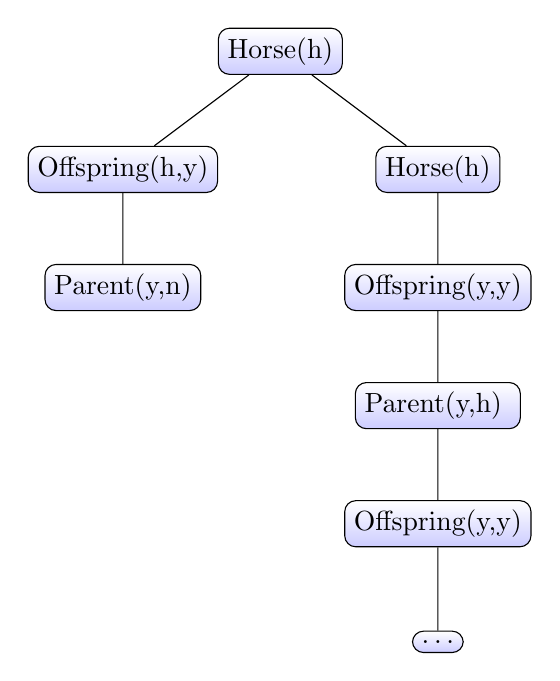
\begin{tikzpicture}[sibling distance = 4cm,
      every node/.style = {shape=rectangle, rounded corners,
        draw, align=center,
        top color=white, bottom color=blue!20}]
      \node{Horse(h)}
        child { node {Offspring(h,y)} 
          child { node {Parent(y,n)} } }
        child { node {Horse(h)}
          child { node {Offspring(y,y)} 
           child { node {Parent(y,h) }
             child {node {Offspring(y,y)}
               child {node{$\ldots$} } } } } };
      \end{tikzpicture}
    \end{enumerate}

\end{enumerate}

\end{document}